\documentclass{beamer}
\usecolortheme{wolverine}

% math stuff
\usepackage{amsmath}
\usepackage{amsthm}
\usepackage{amssymb}
\usepackage{xcolor}

\usepackage{float}
\usepackage{subcaption}

% to insert images
\usepackage{graphicx}

% to correctly insert stressed characters
\usepackage[T1]{fontenc}
\usepackage[utf8]{inputenc}

\usepackage{multirow}

% Bibliography
% \usepackage[style=alphabetic]{biblatex}
% \usepackage[nottoc]{tocbibind}
% \usepackage{bibentry}
% \setcounter{biburllcpenalty}{9000}
% \usepackage{nameref}
% \addbibresource{slides.bib}

% to put links in table of contents
\usepackage{hyperref}
\hypersetup{colorlinks=false, %set true if you want colored links
	linktoc=all,     %set to all if you
}

\usepackage{mathtools}

% Add symbols
% \usepackage{textcomp}

% Add command for Real and Z sets
% \usepackage{dsfont}
% \newcommand{\Rset}{$\mathds{R}$}
% \newcommand{\Zset}{$\mathds{Z}$}

% Code highlighting
% \usepackage{minted}
% \usemintedstyle{perldoc}
% \setminted{
%     frame=single,
%     breaklines,
% }

% tikz figures
\usepackage{tikzit}
\input{style.tikzstyles}

% number rounding
\usepackage{siunitx}
\sisetup{round-mode=places,round-precision=5}

\definecolor{myyellow}{RGB}{225, 225, 0}

\title{Thesis notes}
\date{25th May}

% any code between @(...)@ is escaped back to LaTeX
% \lstset{escapeinside={@(}{)@}}

% algorithms
\usepackage[ruled,vlined]{algorithm2e}
% \newtheorem{theorem}{Theorem}

\begin{document}

\frame{\titlepage}

\begin{frame}[c]
	\frametitle{The Echo Chamber Problem - notation}

	\begin{itemize}
		\item $G = (V, E ^{+}, E ^{-}) $ interaction graph
		\item $ \mathcal{C} $ set of contents
		\item $C \in \mathcal{C} $ content, $\mathcal{T} _{C} $ set of threads
		      associated with $C$. A thread $T \in \mathcal{T} _{C} $ is a
		      subgraph of $G$
		      % So $G = \bigcup _{C
		      % \in \mathcal{C} } \bigcup _{T \in \mathcal{T} _C} T $ union of all
		      % threads of all contents
		\item $U \subseteq V$ subset of users, $T[U]$ subgraph of $T$ induced
		      by $U$. $|T(U)|$ is the number of edges of this subgraph
	\end{itemize}
\end{frame}

\begin{frame}[c]
	\frametitle{The Echo Chamber Problem - notation}
	\begin{itemize}
		\item $\eta(C)$ fraction of negative edges associated with $C$
		      (analogous definition for a thread $T$). Content (or thread)
		      controversial if $\eta \in (\alpha, 1]$
		\item $\hat{\mathcal{C} } \subseteq \mathcal{C} $ set of \textit{controversial}
		      contents

		\item $\mathcal{S} _C (U)$ set of \textit{non controversial} threads
		      induced by $U$, for \textit{controversial} contents, i.e.

			      {\small
				      \begin{equation}
					      \mathcal{S} _{C} (U) = \{ T[U] \; s.t. \; T[U] \; non \;
					      controversial, T \in \mathcal{T} _{C}, C
					      \in \hat{\mathcal{C}}, U \subseteq V\}
				      \end{equation}
			      }
	\end{itemize}

\end{frame}

\begin{frame}[c]
	\frametitle{The Echo Chamber Problem}
	\textbf{Goal}: given an interaction graph $G$, find $U \subseteq V$ maximing

	\begin{equation}
		\xi (U) = \sum^{}_{C \in \hat{\mathcal{C}} } \sum^{}_{T[U] \in S_C (U)}
		(| T^{+} [U] | - | T^{-} [U] |)
	\end{equation}

	where $| T^{-} [U] |$ and $| T^{+} [U] |$ denotes the number of negative
	and positive edges induced in the subgraph, respectively.

	\bigskip

	The set of users maximing the expression is denoted as $\hat{U}$ and the
	corresponding score is $\xi(G)$
\end{frame}

\begin{frame}[c]
	\frametitle{The rounding algorithm}
	\begin{algorithm}[H]
		\SetAlgoLined
		$\hat{G} \leftarrow $ empty graph \;
		$\hat{V} \leftarrow $ vertices of $\hat{G}$ \;
		$S = 0$

		\ForEach{ $e_{ij}^{k} \in \tilde{E}$ }{
		$\hat{V} \leftarrow \hat{V} \bigcup \{ v_{i} \}$ \textbf{if} $v_i
			\not\in \hat{V}$ \;
		$\hat{V} \leftarrow \hat{V} \bigcup \{ v_{j} \}$ \textbf{if} $v_j
			\not\in \hat{V}$ \;

		$S \leftarrow \max(S, \; {\xi}(\hat{V})  )$

		\ForEach{component $C$ in $\hat{G}$}{
			$S \leftarrow \max(S, \; \xi(C)  )$
		}
		}

		\Return S \;

		\caption{Rounding algorithm}
		\label{alg:algorithm_rounding}
	\end{algorithm}
\end{frame}

\begin{frame}[c]
	\frametitle{Example - Original Graph}
	\begin{figure}
		\begin{center}
			\begin{subfigure}[b]{0.4\textwidth}
				\centering
				\tikzfig{tikz/rounding_original_t1}
				\caption{$T_1$}
				\label{fig:rounding-original-t1}
			\end{subfigure}
			\begin{subfigure}[b]{0.4\textwidth}
				\centering
				\tikzfig{tikz/rounding_original_t2}
				\caption{$T_2$}
				\label{fig:rounding-original-t2}
			\end{subfigure}
		\end{center}
		\caption{Example original \emph{Interaction Graph} $G$}
		\label{fig:rounding-original}
	\end{figure}
\end{frame}

\begin{frame}[c]
	\frametitle{Example - Exact solution}
	\begin{figure}
		\begin{center}
			\begin{subfigure}[b]{0.4\textwidth}
				\centering
				\tikzfig{tikz/rounding_integer_t1}
				\caption{$T_1$}
				\label{fig:rounding-integer-t1}
			\end{subfigure}
			\begin{subfigure}[b]{0.4\textwidth}
				\centering
				\tikzfig{tikz/rounding_integer_t2}
				\caption{$T_2$}
				\label{fig:rounding-original-t2}
			\end{subfigure}
		\end{center}
		\caption{Exact solution of the example in \autoref{fig:rounding-original},
			$\alpha = 0.4$}
		\label{fig:rounding-integer}
	\end{figure}
\end{frame}

\begin{frame}[c]
	\frametitle{Example - Relaxation solution}
	\begin{figure}
		\begin{center}
			\begin{subfigure}[b]{0.4\textwidth}
				\centering
				\scalebox{0.8}{
					\tikzfig{tikz/rounding_relaxed_t1}
				}
				\caption{$T_1$, where $z_1 = 0.66$}
				\label{fig:rounding-relaxed-t1}
			\end{subfigure}
			\begin{subfigure}[b]{0.4\textwidth}
				\centering
				\scalebox{0.8}{
					\tikzfig{tikz/rounding_relaxed_t2}
				}
				\caption{$T_2$, where $z_2 = 1.0$}
				\label{fig:rounding-relaxed-t2}
			\end{subfigure}
		\end{center}
		\caption{Solution of the relaxation of $G$ of
			\autoref{fig:rounding-original}, $\alpha = 0.4$}
		\label{fig:rounding-relaxed}
	\end{figure}
\end{frame}

\begin{frame}[c]
	\frametitle{A model for the Echo Chamber Problem}
	Each node has a group assignment and there are probabilities of
	positive and negative edges $\omega _{rs}^{+}  $ and $\omega _{rs}^{+}  $,
	respectively.

	\begin{enumerate}
		\item Generate the \emph{follow} graph $G$ by using a SBM with parameters
		      $\{ \phi _{rs}  \}$.
		\item Each node can be active with probability $\beta_{a}  $
		\item Any active node activates his inactive neighbours in $G$ with
		      probability $\beta_n$
		      % \item Let $a_{i} $ be the number of \emph{active} neighbours of node
		      %     $i$ in $G$ and $m_{i} $ the number of neighbours of node $i$ in
		      %     $G$. Any node inactive from the previous step is activated with
		      %     probability $ \frac{a_i}{m_i} \beta _{n} $
		\item active nodes interact according to the categorical $(\omega _{rs}
			      ^{+}, \omega _{rs} ^{-}, 1 - \omega _{rs} ^{+} - \omega _{rs} ^{-})
		      $ otherwise (at least one of the 2 nodes is inactive) with
		      categorical $(\theta \omega _{rs} ^{+}, \theta \omega _{rs} ^{-}, 1
			      - \theta (\omega _{rs} ^{+} + \omega _{rs} ^{-}))$, $\theta \leq 1$
	\end{enumerate}

\end{frame}

\begin{frame}[c]
	\frametitle{A parametrized model (1)}
	Parameter choice:
	\begin{equation}
		\phi_{rs}  =
		\begin{cases}
			1 \; & \text{if } r = s  \\
			0 \; & \text{otherwise }
		\end{cases}
	\end{equation}
	Users follow other all and only users in the same community.

	\bigskip

	$\beta _{a} = 1$ , $\beta_{n} = 1 $: all users interact on each post.

	\begin{equation}
		\omega_{rs}^{+}   =
		\begin{cases}
			1 - x \; & \text{if } r = s  \\
			x \;     & \text{otherwise }
		\end{cases}
		\omega_{rs}^{-}   =
		\begin{cases}
			x \;     & \text{if } r = s  \\
			1 - x \; & \text{otherwise }
		\end{cases}
	\end{equation}
\end{frame}

\begin{frame}[c]
	\frametitle{A parametrized model (2)}

	The tests have been carried on very small graphs since the exact model was
	also used, $10$ nodes per community and $3$ threads.

\end{frame}

\begin{frame}[c]
	\frametitle{A parametrized model - results}

	Even in absence of noise the approximation algorithm is not able to cluster all
	nodes correctly, differently from the exact MIP model.

	\begin{figure}
		\begin{center}
			\begin{subfigure}[b]{0.3\textwidth}
				\centering
				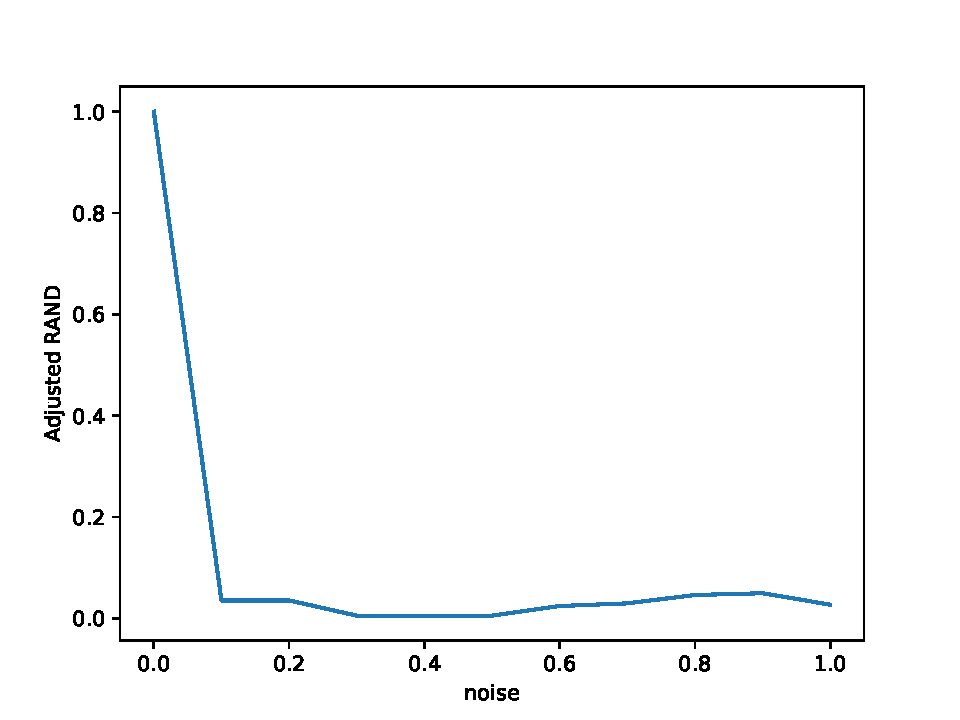
\includegraphics[width=\textwidth]{out/synthetic_exact/model2_noise_adj_rand.pdf}
				\caption{Adj RAND, MIP}
				\label{fig:out/synthetic_exact/model2_sigmas_adj_rand.pdf}
			\end{subfigure}
			\begin{subfigure}[b]{0.3\textwidth}
				\centering
				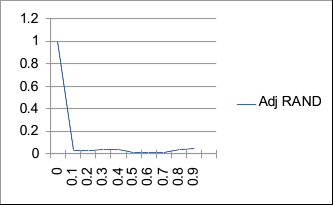
\includegraphics[width=\textwidth]{out/synthetic_approximation/adj.png}
				\caption{Adj RAND, approx.}
				\label{fig:adj-rand-appr1}
			\end{subfigure}
		\end{center}
		\begin{center}
			\begin{subfigure}[b]{0.3\textwidth}
				\centering
				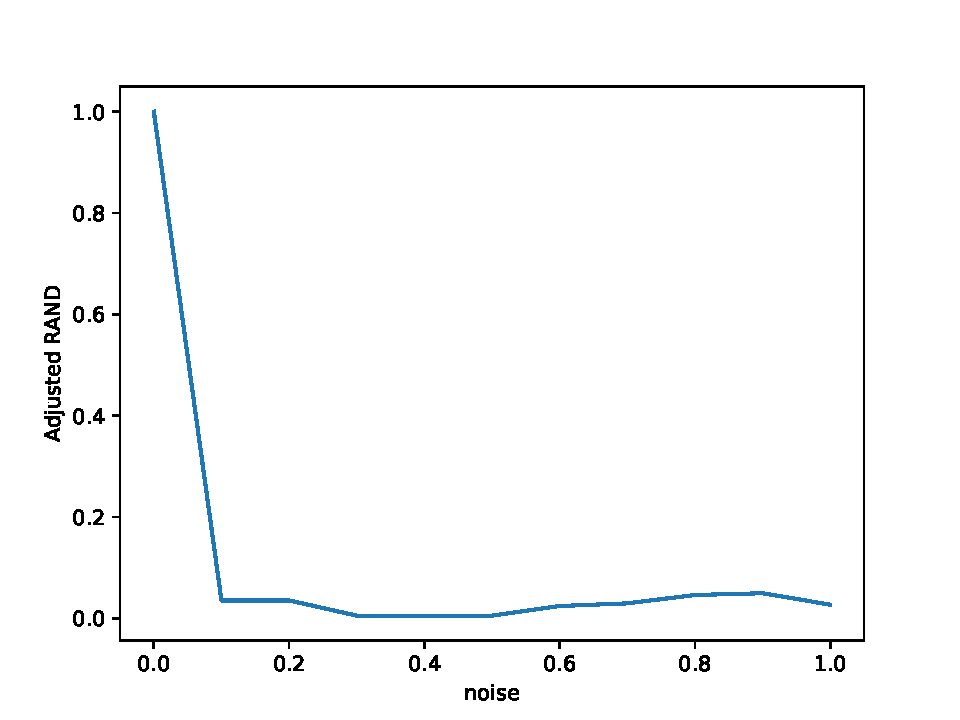
\includegraphics[width=\textwidth]{out/synthetic_exact/model2_noise_adj_rand.pdf}
				\caption{Jaccard, MIP}
				\label{fig:out/synthetic_exact/model2_sigmas_jaccard.pdf}
			\end{subfigure}
			\begin{subfigure}[b]{0.3\textwidth}
				\centering
				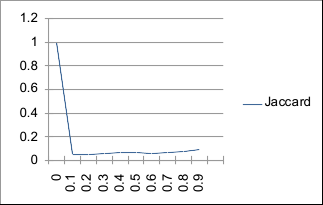
\includegraphics[width=\textwidth]{out/synthetic_approximation/jacc.png}
				\caption{Jaccard, approx.}
				\label{fig:jacc-appr1}
			\end{subfigure}
		\end{center}
	\end{figure}

\end{frame}

% \begin{frame}[c]
%     \frametitle{A parametrized model - results}
%
%     MIP is also more robust to noise than the other variants of the problem.
%
%     \begin{figure}
%         \begin{center}
%             \begin{subfigure}[t]{0.3\textwidth}
%                 \centering
%                 \includegraphics[width=\textwidth]{out/synthetic_densest_nc/model2_sigmas_adj_rand.pdf}
%                 \caption{Adj RAND, Densest subgraph on Threads}
%                 \label{fig:out/synthetic_densest_nc/model2_sigmas_adj_rand.pdf}
%             \end{subfigure}
%             \begin{subfigure}[t]{0.3\textwidth}
%                 \centering
%                 \includegraphics[width=\textwidth]{out/synthetic_o2_bff/model2_sigmas_adj_rand.pdf}
%                 \caption{Adj RAND, O$^{2}$-BFF}
%                 \label{fig:adj-rand-o2_bff1}
%             \end{subfigure}
%         \end{center}
%         \begin{center}
%             \begin{subfigure}[t]{0.3\textwidth}
%                 \centering
%                 \includegraphics[width=\textwidth]{out/synthetic_densest_nc/model2_sigmas_jaccard.pdf}
%                 \caption{Jaccard, Densest subgraph on Threads}
%                 \label{fig:out/synthetic_densest_nc/model2_sigmas_jaccard.pdf}
%             \end{subfigure}
%             \begin{subfigure}[t]{0.3\textwidth}
%                 \centering
%                 \includegraphics[width=\textwidth]{out/synthetic_o2_bff/model2_sigmas_jaccard.pdf}
%                 \caption{Jaccard, O$^{2}$-BFF}
%                 \label{fig:jacc-o2_bff1}
%             \end{subfigure}
%         \end{center}
%     \end{figure}
%
% \end{frame}

\begin{frame}[c]
	\frametitle{Analyzing @nytimes results}
	A graph from @nytimes, with 500 contents

	$\alpha $ chosen as the median of the $\eta$ of the contents, $\alpha =
		0.44$.

	The graph contains $\approx$ 83000 nodes and $\approx$ 120000 edges,
	$\xi(G) \approx 30000 $ on 27000
	vertices and define $\approx 1500$ components. In the original graph there
	were 829 components.

	\begin{itemize}
		\item Average shortest path length: 1.94
		\item Median shortest path length: 1.0
		\item Average degree: 1.35
		\item Contributing threads: 2200
		\item Number of threads in the graph: 6246
	\end{itemize}

\end{frame}

\begin{frame}[c]
	\frametitle{Analyzing @nytimes results}

	Contents that contribute the most to the score:
	\begin{figure}[htpb]
		\centering
		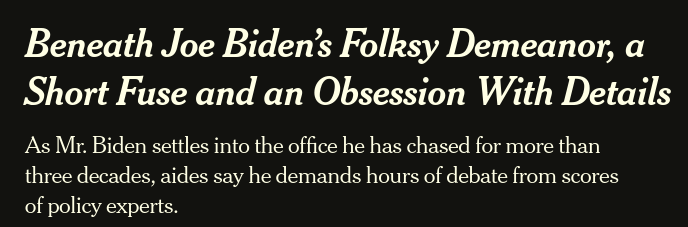
\includegraphics[width=0.5\textwidth]{out/nytimes700/results/content1.png}
		\caption{3047}
		\label{fig:name}
	\end{figure}
	\begin{figure}[htpb]
		\centering
		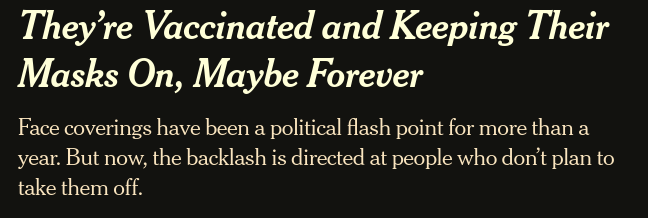
\includegraphics[width=0.5\textwidth]{out/nytimes700/results/content2.png}
		\caption{2431}
		\label{fig:name}
	\end{figure}
	\begin{figure}[htpb]
		\centering
		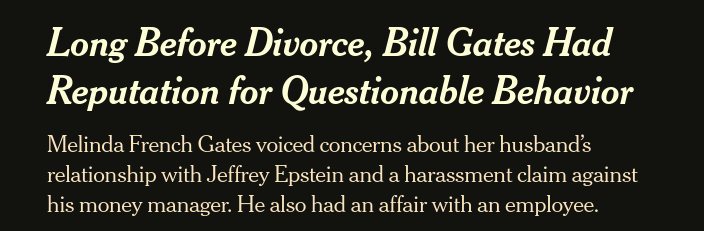
\includegraphics[width=0.5\textwidth]{out/nytimes700/results/content3.png}
		\caption{1922}
		\label{fig:name}
	\end{figure}


\end{frame}

\begin{frame}[c]
	\frametitle{Analyzing @nytimes results - examples}
	It is in general not easy to easily distinguish Echo Chamber since
	\begin{itemize}
		\item components are very small and so there are very few comments
		\item not all edges are related to the same thread
		\item comments are reply to other comments which are missing in the
		      Echo chamber, making it difficult to catch up with the discussion
	\end{itemize}

	The resulting communities and thread sometimes contains also noise
	introduced by images and people speaking languages different from English.
\end{frame}

\begin{frame}[c]
	\frametitle{Analyzing @nytimes results - examples}
	Usually echo chambers contains 2 or 3 comments which show the same opinion
	while the rest of the comments and users in the chamber do not really show
	their alignment. Example, about Bill Gates's divorce:

	\begin{enumerate}
		\item B to A: "Well this is not the problem, the main one is his
		      friendship with Epstein and many of his travels in the Lolita's
		      xxxpress"
		\item C to A: "Fantasme ! ?"

		\item D to A: "don't worry his wife will have a big slice of his cake!"
		\item E to A: "Philanthropie..."
		\item F to A: "Wait till his lawyer kicks up some juicy bits"
	\end{enumerate}
\end{frame}

\end{document}
